\documentclass{beamer}
\usepackage{graphicx}
\usepackage{array}
\usepackage{amsmath, nccmath}
\usepackage[utf8]{inputenc}
\usepackage[T1]{fontenc}
\usepackage[french]{babel}

\usetheme{Boadilla}

%%% Metadata %%%
\title[Attaques sur HTTPS]{Attaque Man-In-The-Middle de HTTPS}
\subtitle{SSLStrip, HTTPS-Interception...}
\author[S. Duret - A. Risi - B. Guevel]{Simon Duret\\Amélie Risi\\Brendan Guevel}
\institute[]{Université de Bordeaux}
\date{14 Mai 2018}

\begin{document}

%%% Title page %%%
\begin{frame}
	\titlepage
\end{frame}

\begin{frame}{Introduction}
    {\Large \centerline{HTTP est \textbf{le} protocole central du net}}

    Assure la transmission des données entre un client et un serveur \\
    % Dire à l'oral que client = navigateur généralement, et serveur = site web
    -> Problème : Tout le traffic est en clair \\
    % Donner des exemples à l'oral : interception du wifi, ou physiquement au niveau du cable ethernet, ...
    HTTPS : Extension de HTTP pour chiffrer un échange entre un client et un serveur \\
    -> Assure la confidentialité des données (mot de passe, numéro de carte bancaire, ...) \\

    Malgré ce chiffrement, des attaques restent possibles...

\end{frame}

\begin{frame}{Introduction}
    {\Large \centerline{Plan}}

    1. Fonctionnement de HTTP et HTTPS \\
    2. Etat de l'art des attaques sur SSL/TLS \\
    3. Presentation de notre implémentation \\
        a. Environnement qemunet \\
        b. SSLstrip \\
        c. SSLstrip+ \\
        d. SSLstrip NTP \\
        e. HTTPS interception \\

\end{frame}

\section{Fonctionnement de HTTP}

\begin{frame}{Fonctionnement de HTTP}
    Procotole de communication client-serveur \\
    Le client demande une ressource à un serveur via une requête HTTP \\
    % Généralement une page html
    Le serveur envoie au client la ressource demandée en réponse \\
    Un navigateur web permet d'automatiser ce processus \\
    De plus ce dernier permet d'afficher la page avec la mise en forme html/css

\end{frame}

\begin{frame}{Exemple d'une requête HTTP}
    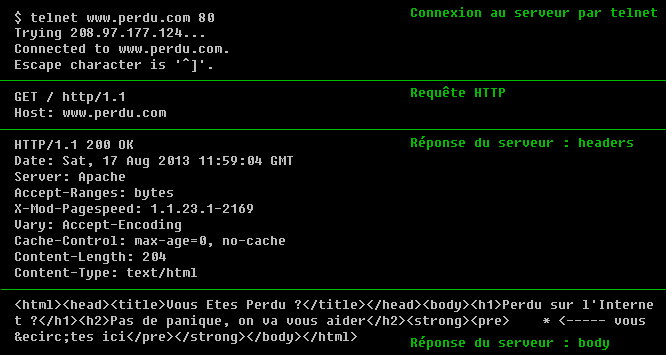
\includegraphics[scale=0.50]{../medias/perdu.png}
    % Faire une petite démo en live (avec la même requête)
\end{frame}

\begin{frame}{HTTPS : la version chiffrée de HTTP}
    S pour secure \\
    C'est un deuxième protocole qui est rajouté par dessus HTTP \\
    Historiquement SSL, aujourd'hui remplacé par TLS \\
    Applique un chiffrement sur toute la communication HTTP \\

    Limitation : un attaquant peut toujours voir l'IP/port de destination (nécessaire pour TCP/IP)
\end{frame}


\section{Etat de l'art}

\begin{frame}{Attaques sur HTTPS}
    HTTPS est la combinaison de deux protocoles très différents \\
    -> Un attaquant a plus de matière pour attaquer une communication \\
    
\end{frame}

\begin{frame}{Historique des attaques sur SSL/TLS}
    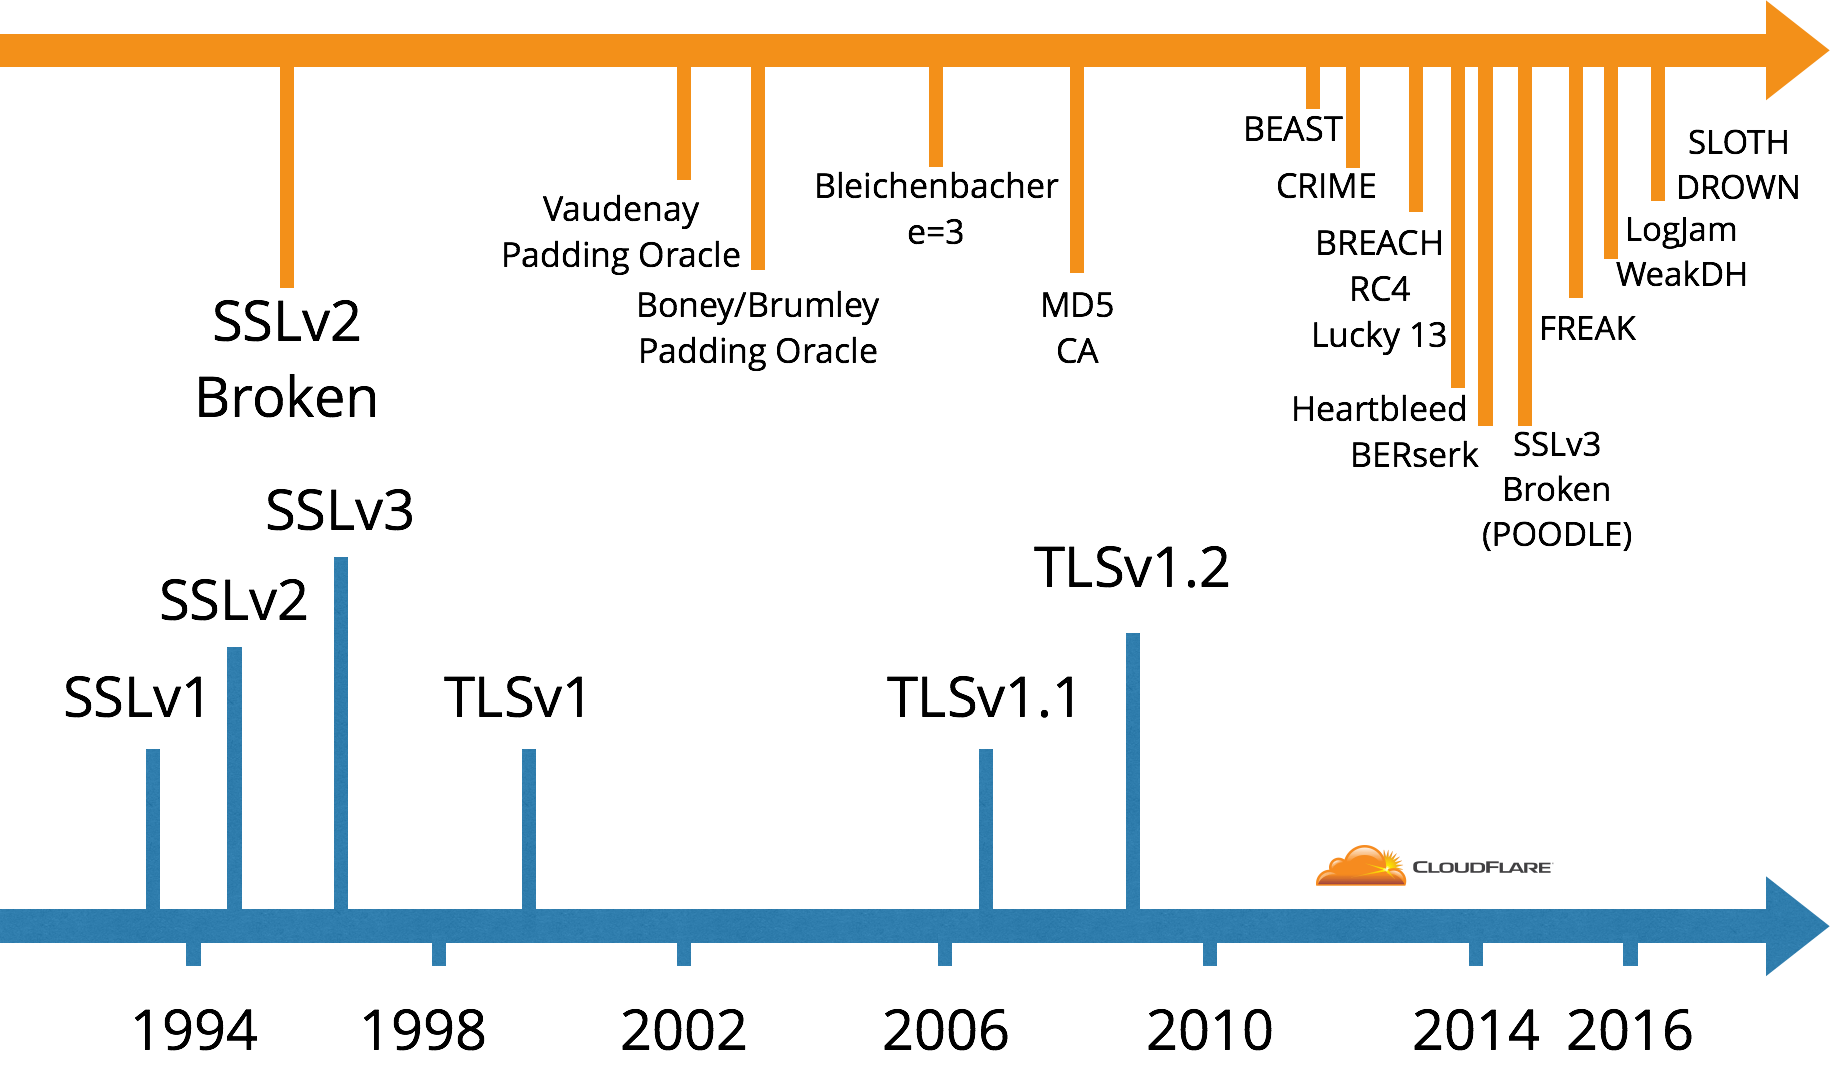
\includegraphics[scale=0.19]{../medias/history-tls-attacks.png}
\end{frame}

\section{Environnement}

\begin{frame}{Environnement}
    \begin{block}{Qemunet}
		Outil pour créer un réseau virtuel
    \end{block}
\end{frame}

\begin{frame}{Topologie}
    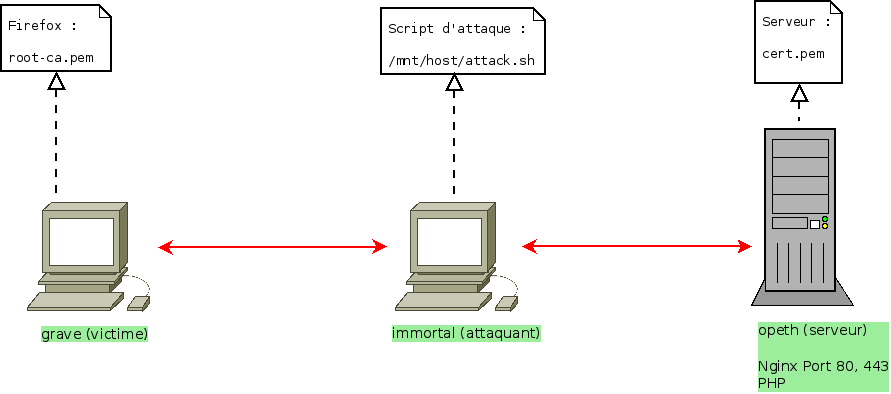
\includegraphics[scale=0.4]{../medias/topology.png}
\end{frame}

\section{Attaque SSLstrip}

\begin{frame}{Fonctionnement d'un lien dans une page html}

\end{frame}

\begin{frame}{Attaque SSLstrip}
    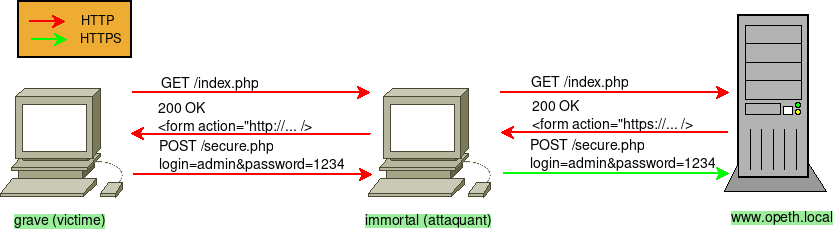
\includegraphics[scale=0.4]{../medias/sslstrip/attack.png}
\end{frame}

\section{Attaque SSLstrip+}

\begin{frame}{Fonctionnement de DNS}
\end{frame}

\begin{frame}{Attaque SSLstrip+}
    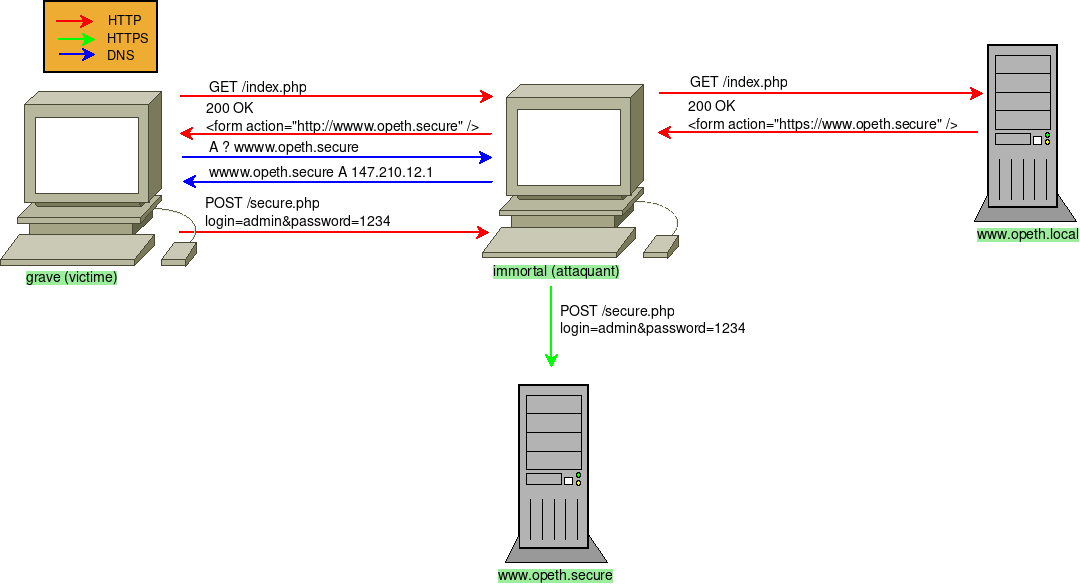
\includegraphics[scale=0.32]{../medias/sslstrip2/attack.png}
\end{frame}

\section{Attaque SSLstrip NTP}

\begin{frame}{Fonctionnement de NTP}
\end{frame}

\begin{frame}{Attaque SSLstrip NTP}
    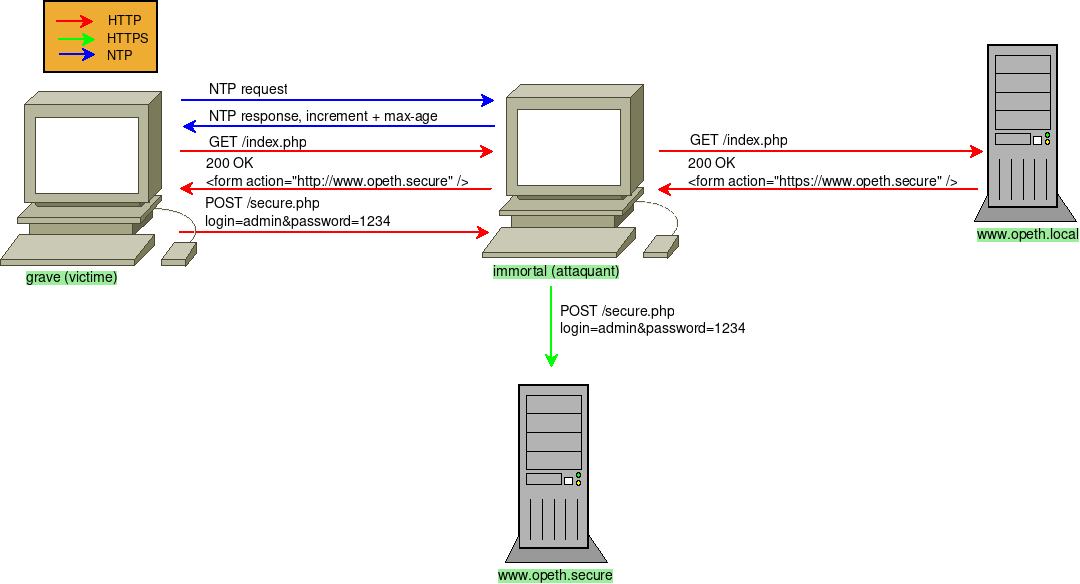
\includegraphics[scale=0.32]{../medias/sslstrip-ntp/attack.png}
\end{frame}

\section{Attaque HTTPS interception}

\begin{frame}{Certificat numérique}
    -> Permet d'authentifier la communication \\
    -> Sur internet, cela sert essentiellement à s'assurer de l'identité du serveur \\
    -> Nécessité d'une authorité de certification (un tiers) \\
\end{frame}

\begin{frame}{Attaque HTTPS interception}
    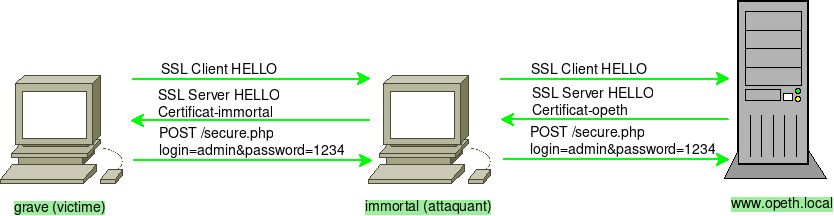
\includegraphics[scale=0.4]{../medias/https-interception/attack.png}
\end{frame}







\end{document}
